\documentclass[a4paper]{exam}


\usepackage[table]{xcolor}
\usepackage[export]{adjustbox}
\usepackage{clrscode3e}
\usepackage{amsmath,amssymb,amsthm}
\usepackage{geometry}
\usepackage{graphicx}
\usepackage{hyperref}
\usepackage{pythonhighlight}
\usepackage{tabularx}


\printanswers
\addpoints
\title{Homework Assignment 1}
\author{CS/CE 412/471 Algorithms: Design and Analysis, Spring 2025}
\date{\numquestions\ problems, \numpoints\ points}

% \qformat{{\large\bf \thequestion. \thequestiontitle}\hfill}
\boxedpoints

\begin{document}
\maketitle
\thispagestyle{empty}


\includegraphics[trim=0 5cm 0 1cm, clip, width=\textwidth]{title}
\begin{questions}
  
\question[10]
  Sort the order of growth of the following functions and justify your solution.
  \[
    f_1(n) = 7n,\quad f_2(n) = \lg n^{\lg n},\quad f_3(n) = n^{\lg n},\quad f_4(n) = n^2\lg n
  \]
  \[
    f_5(n) = \left(\frac{n}{2}\right)^{\frac{n}{2}},\quad f_6(n) = 3^{n^3},\quad f_7(n) = n^{\lg 3},\quad f_8(n) = n^2
  \]
  If some have the same asymptotic growth, then be sure to indicate that. As usual, $\lg$ indicates a base of 2.
    \begin{solution}
      An initial ordering from lowest to highest order of growth can be established based on coefficients and powers of $n$.
      \[ \begin{array}{c|c|c|c}
        f_1& f_7&f_8&f_4\\\hline
        7n& n^{\lg3}&n^2&n^2\lg n
      \end{array} \]
      Since exponential functions grow faster than polynomials, we can include $f_6$.
      \[ \begin{array}{c|c|c|c|c}
        f_1& f_7&f_8&f_4&f_6\\\hline
        7n& n^{\lg3}&n^2&n^2\lg n&3^{n^3}
      \end{array} \]
      It remains to insert $f_2,f_3,f_5$ into the ordering.

      We show that $f_2$ grows slower than $f_1$.

      Consider $\lim\limits_{n\to\infty}\frac{f_2(n)}{f_1(n)}=\lim\limits_{n\to\infty}\frac{\lg n^{\lg n}}{7n} = \lim\limits_{n\to\infty}\frac{(\lg n)(\lg n)}{7n} =\lim\limits_{n\to\infty}\frac{(\lg n)^2}{7n} $.

      Applying L'Hopital's rule, this becomes $\lim\limits_{n\to\infty}\frac{(2\lg n)(1/n)}{7}=\lim\limits_{n\to\infty}\frac{2\lg n}{7n}$.

      As the denominator grows faster than the numerator, the above limit is 0.

      We include $f_2$ in the ordering as follows.
      \[ \begin{array}{c|c|c|c|c|c}
        f_2 & f_1& f_7&f_8&f_4&f_6\\\hline
        \lg n^{\lg n} & 7n& n^{\lg3}&n^2&n^2\lg n&3^{n^3}
      \end{array} \]
    As $f_3(n)=n^{\lg n}$ is exponential in $n$, it dominates $f_4(n)=n^2\lg n$ which is polynomial in $n$.

    The relation of $f_3(n)=n^{\lg n}$ to $f_6(n)=3^{n^3}$ needs to be explored.

    Let us compare their logarithms: $\lg f_3(n) = (\lg n)^2$ and $\lg f_6(n) = n^3\lg 3$.

      We include $f_2$ in the ordering as follows.
      \[ \begin{array}{c|c|c|c|c|c|c}
        f_2 & f_1& f_7&f_8&f_4&f_3&f_6\\\hline
        \lg n^{\lg n} & 7n& n^{\lg3}&n^2&n^2\lg n& n^{\lg n} &3^{n^3}
      \end{array} \]
    $f_5(n) = \left(\frac{n}{2}\right)^{\frac{n}{2}}$ remains.

    The power of $n$ in $f_5$ is linear in $n$ and logarithmic term in $f_3$.

    Comparing $f_5$ to $f_6$, let us again compare logarithms.

    $\lg f_5(n) = \frac{n}{2}\lg\frac{n}{2}$ and $\lg f_6(n) = n^3\lg 3$.
      We include $f_2$ in the ordering as follows.
      \[ \begin{array}{c|c|c|c|c|c|c|c}
        f_2 & f_1& f_7&f_8&f_4&f_3&f_5&f_6\\\hline
        \lg n^{\lg n} & 7n& n^{\lg3}&n^2&n^2\lg n& n^{\lg n} &\left(\frac{n}{2}\right)^{\frac{n}{2}}&3^{n^3}
      \end{array} \]
  \end{solution}

\question
  Prove or disprove each of the following:
  \begin{parts}
  \part[5] $f(n) = \Theta\left( f\left(\frac{n}{4}\right)\right)$
    \begin{solution}
      Can be proved case-wise by considering polynomial and exponential functions, $f$.
    \end{solution}
  \part[5] $2^n = o(2^{\frac{n}{2}})$ (i.e. $2^n = O(2^{\frac{n}{2}})$ and $2^n \ne \Theta(2^{\frac{n}{2}})$)
    \begin{solution}
      \begin{proof} The claim is false.
        
        We provide a direct proof.

        Let $N=2^n$.

      Then the claim becomes, $N=O(\sqrt{N})$ and $N\ne \Theta(\sqrt{N})$.

      Clearly, the claim $N=O(\sqrt{N})$ is false.

      Therefore the given claim is false.
    \end{proof}
  \end{solution}
  \part[5] $\Theta(f(n)) + \Theta(g(n))=\Theta(f(n)+g(n))$
    \begin{solution}
      \begin{proof} The claim is true.

        We show that LHS equals RHS.
        
      Applying the definition of $\Theta$,
      \[
        c_1f(n) \le \Theta(f(n)) \le c_2f(n) \;\text{ and }\; d_1g(n) \le \Theta(g(n)) \le d_2g(n).
      \]
      Adding the two, 
      \[
        c_1f(n) + d_1g(n) \le \Theta(f(n)) + \Theta(g(n)) \le c_2f(n) + d_2g(n).
      \]
      Then,
      \[
        \Theta(f(n)) + \Theta(g(n)) \ge c_1f(n) + d_1g(n) \ge \min(c_1,d_1)(f(n) + d_1g(n)).
      \]
      That is, $\Theta(f(n)) + \Theta(g(n)) = \Omega(f(n)+g(n))$.

      Similarly,
      \[
        \Theta(f(n)) + \Theta(g(n)) \le c_2f(n) + d_2g(n) \le \max(c_2,d_2)(f(n) + d_1g(n)).
      \]
      That is, $\Theta(f(n)) + \Theta(g(n)) = \O(f(n)+g(n))$.

      Then, $\Theta(f(n)) + \Theta(g(n)) = \Theta(f(n)+g(n))$.
    \end{proof}
  \end{solution}
  \end{parts}
% \question
% Let $L$ be an array $L[1:n]$. The number of inversions in $L$ is the number of pairs $i < j$ such that $L[i] > L[j]$. Prove or disprove that counting the number of inversions requires at least $\Theta(n \lg n)$ comparisons in the worst case.

\question You are given 2 problems below. You need to design an efficient algorithm for each of them. Specifically,

  \begin{enumerate}
    \renewcommand{\theenumi}{\roman{enumi}} % Set enumeration to a, b, c...
    \item Clearly state the problem. For example, see how the sorting problem is stated on the first page of Chapter 1 of CLRS.
    \item Describe your algorithm. Follow the pseudocode conventions listed in Section 2.1 of CLRS. \textit{Do not} use programming language features, e.g. \pyth{list.append().}
    \item Illustrate, in any suitable manner, e.g. as in Section 2.1 in CLRS, a run of your algorithm on a sample input.
    \item Describe the best and worst case for your algorithm.
    \item Describe an input, if any, on which your algorithm may not work correctly.
    \item Provide a time complexity analysis of your algorithm in terms of input size $n$ using asymptotic notation.
    \end{enumerate}

  \begin{parts}
  \part[10] Given a number, $x$, and an array, $A$, containing $n$ numbers, decide if the array contains two numbers $a$ and $b$ such that $a+b = x$.
    \begin{solution}
    \begin{enumerate}
    \renewcommand{\theenumi}{\roman{enumi}}
    \item
      \begin{tabularx}{.8\textwidth}{l|X}
        Input & An array, $A$, of numbers, its size, $n$, and a number, $x$.\\\hline
        Output & \texttt{True} if the array contains two numbers $a$ and $b$ such that $a+b = x$, \texttt{False} otherwise.
      \end{tabularx}
    \item
\begin{codebox}
\Procname{$\proc{Pair-Exists}(A, n, x)$}
\li $S \gets $ empty set
\li \For $i \gets 1$ \To $n$
\Do
\li $a \gets A[i]$
\li $b \gets x - a$
\li \If $b \in S$
\Do
\li \Return \const{true} 
\End
\li $S \gets S \bigcup \{a\}$
\End
\li \Return \const{false}
\End
\end{codebox}
      
    \item       (a)
      \begin{tabular}{l}
      \begin{tabular}{|*4{c|}}
        \hline
        \cellcolor{yellow}5&4&3&3\\\hline
      \end{tabular}\\
        $S = \{\}$\\
        \colorbox{red!50}{$b = 1$}
      \end{tabular}
      (b)
      \begin{tabular}{l}
      \begin{tabular}{|*4{c|}}
        \hline
        5&\cellcolor{yellow}4&3&3\\\hline
      \end{tabular}\\
        $S = \{5\}$\\
        \colorbox{red!50}{$b = 2$}
      \end{tabular}
      (c)
      \begin{tabular}{l}
      \begin{tabular}{|*4{c|}}
        \hline
        5&4&\cellcolor{yellow}3&3\\\hline
      \end{tabular}\\
        $S = \{5,4\}$\\
        \colorbox{red!50}{$b = 3$}
      \end{tabular}\\
      (d)
      \begin{tabular}{l}
      \begin{tabular}{|*4{c|}}
        \hline
        5&4&3&\cellcolor{yellow}3\\\hline
      \end{tabular}\\
        $S = \{5,4,3\}$\\
        \colorbox{green!50}{$b = 3$}
      \end{tabular}

      A call to $\proc{Pair-Exists}(A, 4, 6)$. \colorbox{yellow}{$a$} is shown for each interaction along with the current state of $S$ and the required $b$. (a) In the first iteration, \colorbox{yellow}{$a=5$}. The value of \colorbox{red!50}{$b=1$} is not found in $S$, which is then updated. (b-c) The algorithm proceeds similarly. (d) The value of \colorbox{green!50}{$b=3$} is found in $S$. The algorithm returns \const{true} and terminates.

    \item The best case is when the first two elements of $A$ add up to $x$. The worst case is when no such pair exists in $A$.
    \item The algorithm will work correctly provided all types are as expected.
    \item All lines take constant time with possible uncertainty about set operations. If the set is implemented using a hash table, its operations will take constant time (amortized). In the worst case, no pair is found and the \For\ loop on line 2 completes. The time complexity is therefore $O(n)$.
    \end{enumerate}
    \end{solution}
  \part[10] Given $k$ sorted lists containing a total of $n$ numbers, combine them to create a single sorted list of the $n$ numbers.
    \begin{solution} 
  \begin{enumerate}
    \renewcommand{\theenumi}{\roman{enumi}}
    \item
      \begin{tabularx}{.9\textwidth}{l|X}
        Input & $k$ sorted arrays, $A_1, A_2,\twodots,A_k$, of numbers where $|A_i|=n_i, 1\le i\le k$, and $\sum_in_i=n$.\\\hline
        Output & A sorted array, $A$, containing all the numbers in $A_1, A_2,\twodots,A_k$.
      \end{tabularx}
    \item
\begin{codebox}
\Procname{$\proc{k-way-merge}(A_1, A_2, \twodots, A_k, k, n)$}
\li \Comment assumes 1-indexing
\li $A \gets $ array of size $n$ \Comment final array
\li $\id{idx} \gets $ array of $k$ $1$s \Comment index in each $A_i$
\li \For $j \gets 1$ \To $n$
\Do
\li \Comment get smallest number from $A_i$s to add to $A$
\li $m\gets \infty$
\li \For $i \gets 1$ \To $k$
\Do
\li \If $\id{idx}[i]\le \attrib{A_i}{length}$ and $A_i[\id{idx}[i]] < m$
\Then
\li $m\gets A_i[\id{idx}[i]]$
\End
\End
\li \Comment update index for identified $A_i$
\li \For $i \gets 1$ \To $k$
\Do
\li \If $\id{idx}[i]\le \attrib{A_i}{length}$ and $A_i[\id{idx}[i]] \isequal m$
\Then
\li $\id{idx}[i] \gets \id{idx}[i] + 1$
\li break
\End
\End
\li $A[j]\gets m$
\End
\li \Return $A$
\end{codebox}
      
    \item       (a)
      \begin{tabular}{l}
      $A_1$\begin{tabular}{|*3{c|}}
        \hline
        \textbf{3}&\cellcolor{yellow}10&17\\\hline
      \end{tabular}\\ \\
      $A_2$\begin{tabular}{|*2{c|}}
        \hline
        \cellcolor{yellow}4&6\\\hline
      \end{tabular}\\ \\
        $A_3$\begin{tabular}{|*2{c|}}
        \hline
        \cellcolor{yellow}11&20\\\hline
      \end{tabular}\\ \\
      $A$\begin{tabular}{|*7{c|}}
        \hline
        \cellcolor{green!50}3& & & & & & \\\hline
      \end{tabular}
      \end{tabular}
       (b)
      \begin{tabular}{l}
        $A_1$\begin{tabular}{|*3{c|}}
        \hline
        3&\cellcolor{yellow}10&17\\\hline
      \end{tabular}\\ \\
        $A_2$\begin{tabular}{|*2{c|}}
        \hline
        \textbf{4}&\cellcolor{yellow}6\\\hline
      \end{tabular}\\ \\
        $A_3$\begin{tabular}{|*2{c|}}
        \hline
        \cellcolor{yellow}11&20\\\hline
      \end{tabular}\\ \\
        $A$\begin{tabular}{|*7{c|}}
        \hline
        3& \cellcolor{green!50}4& & & & & \\\hline
      \end{tabular}
      \end{tabular}
       (c)
      \begin{tabular}{l}
        $A_1$\begin{tabular}{|*3{c|}}
        \hline
        3&\cellcolor{yellow}10&17\\\hline
      \end{tabular}\\ \\
        $A_2$\begin{tabular}{|*2{c|}}
        \hline
        \rowcolor{red!50}
        4&\textbf{6}\\\hline
      \end{tabular}\\ \\
        $A_3$\begin{tabular}{|*2{c|}}
        \hline
        \cellcolor{yellow}11&20\\\hline
      \end{tabular}\\ \\
        $A$\begin{tabular}{|*7{c|}}
        \hline
        3& 4& \cellcolor{green!50}6 & & & & \\\hline
      \end{tabular}
      \end{tabular}\\[5pt]
      \centerline{\rule{250pt}{.5pt}}
      
       (d)
      \begin{tabular}{l}
        $A_1$\begin{tabular}{|*3{c|}}
        \hline
        3&\textbf{10}&\cellcolor{yellow}17\\\hline
      \end{tabular}\\ \\
        $A_2$\begin{tabular}{|*2{c|}}
        \hline
        \rowcolor{red!50}
        4&6\\\hline
      \end{tabular}\\ \\
        $A_3$\begin{tabular}{|*2{c|}}
        \hline
        \cellcolor{yellow}11&20\\\hline
      \end{tabular}\\ \\
        $A$\begin{tabular}{|*7{c|}}
        \hline
        3& 4& 6 & \cellcolor{green!50}10& & & \\\hline
      \end{tabular}
      \end{tabular}
       (e)
      \begin{tabular}{l}
        $A_1$\begin{tabular}{|*3{c|}}
        \hline
        3&10&\cellcolor{yellow}17\\\hline
      \end{tabular}\\ \\
        $A_2$\begin{tabular}{|*2{c|}}
        \hline
        \rowcolor{red!50}
        4&6\\\hline
      \end{tabular}\\ \\
        $A_3$\begin{tabular}{|*2{c|}}
        \hline
        \textbf{11}&\cellcolor{yellow}20\\\hline
      \end{tabular}\\ \\
        $A$\begin{tabular}{|*7{c|}}
        \hline
        3& 4& 6 & 10& \cellcolor{green!50}11 & & \\\hline
      \end{tabular}
      \end{tabular}\\[5pt]
      \centerline{\rule{250pt}{.5pt}}
      
       (f)
      \begin{tabular}{l}
        $A_1$\begin{tabular}{|*3{c|}}
        \hline
        \rowcolor{red!50}
        3&10&\textbf{17}\\\hline
      \end{tabular}\\ \\
        $A_2$\begin{tabular}{|*2{c|}}
        \hline
        \rowcolor{red!50}
        4&6\\\hline
      \end{tabular}\\ \\
        $A_3$\begin{tabular}{|*2{c|}}
        \hline
        11&\cellcolor{yellow}20\\\hline
      \end{tabular}\\ \\
        $A$\begin{tabular}{|*7{c|}}
        \hline
        3& 4& 6 & 10& 11 & \cellcolor{green!50}17& \\\hline
      \end{tabular}
      \end{tabular}
       (g)
      \begin{tabular}{l}
        $A_1$\begin{tabular}{|*3{c|}}
        \hline
        \rowcolor{red!50}
        3&10&17\\\hline
      \end{tabular}\\ \\
        $A_2$\begin{tabular}{|*2{c|}}
        \hline
        \rowcolor{red!50}
        4&6\\\hline
      \end{tabular}\\ \\
        $A_3$\begin{tabular}{|*2{c|}}
        \hline
        \rowcolor{red!50}
        11&\textbf{20}\\\hline
      \end{tabular}\\ \\
        $A$\begin{tabular}{|*7{c|}}
        \hline
        3& 4& 6 & 10& 11 & 17&\cellcolor{green!50}20 \\\hline
      \end{tabular}
      \end{tabular}\\[5pt]
      
      A call to $\proc{k-way-merge}$ with $k=3, n=7$, and $A_1,A_2,A_3$ as shown. (a) The elements in the $A_i$s as indicated by \id{idx} are in yellow. The first element from $A_1$ is chosen as $m$ and copied to $A$ and its index has advanced. (b) The first element of $A_2$ is copied to $A$. (c) The second element of $A_2$ is copied to $A$. $A_2$ is now exhausted. (d-f) The algorithm proceeds similarly. (g) $A$ gets its last element. All $A_i$s are exhausted.

    \item Very few lines depend on a conditional. So the best case and worst case are similar. The execution of Line 9 depends on a condition and the \For loop on Line 11 may break before completion. But that will have little impact on the overall running time.
    \item The algorithm will work correctly provided all types and inputs are as expected.
    \item Assuming memory allocation to take constant time, all lines take constant time. The outer \For loop (line 4) runs in time linear in $n$. The inner \For loop on line 7 runs in time linear in $k$. The inner \For loop on line 11 runs in time linear in $k$ or less, depending on the input. However, the time for the body of the outer \For loop on line 4 is already determined by the inner \For loop on line 7. The overall time complexity is therefore $\Theta(nk)$.
    \end{enumerate}
    \end{solution}
  \end{parts}
  
\question For each of the following recurrences, derive a solution to the recurrence (show your working) and compare your solution with that obtained through the master theorem (show how it applies). 
  \begin{parts}
  \part[5] $T(n) = 2T\left(\frac{n}{4}\right) + 1$
    \begin{solution}
      Unrolling leads to the pattern, $T(n)=2^iT(\frac{n}{4^i}) + \sum_{j=0}^{i-1}2^j = 2^iT(\frac{n}{4^i}) + 2^i-1$.

      The base case occurs at $i=\log_4n$.

      Substituting, $T(n) = 2^{\log_4n}c +2^{\log_4n} - 1 = $ \colorbox{yellow}{$\Theta(\sqrt{n})$}.

      In terms of the master theorem, $f(n)=n^0$ and $n^{\log_ba}=n^{0.5}$.

      Case 1 of the theorem applies, $f(n) = O(n^{\log_ba-\epsilon})$. One solution is $\epsilon=0.5$.

      Then, $T(n)=\Theta(n^{\log_ba})=$ \colorbox{yellow}{$\Theta(\sqrt{n})$}, as obtained above.
    \end{solution}
  \part[5] $T(n) = 2T\left(\frac{n}{4}\right) + n$
    \begin{solution}
      Unrolling leads to the pattern, $T(n)=2^iT(\frac{n}{4^i}) + n\sum_{j=0}^{i-1}2^{-j} = 2^iT(\frac{n}{4^i}) + n(2 - 2^{1-i})$.

      The base case occurs at $i=\log_4n$.

      Substituting, $T(n) = 2^{\log_4n}c +n(2-2^{1-\log_4n}) = c\sqrt{n}+2n-2\sqrt{n}=$ \colorbox{yellow}{$\Theta(n)$}.

      In terms of the master theorem, $f(n)=n^1$ and $n^{\log_ba}=n^{0.5}$.

      Case 3 of the theorem applies, $f(n) = \Omega(n^{\log_ba+\epsilon})$. One solution is $\epsilon=0.5$.

      Additionally, for the regularity condition, $2f(\frac{n}{4})\le cf(n) \implies \frac{2n}{4}\le cn$.

      One solution is $c=\frac{1}{2}$.

      Then, $T(n)=\Theta(f(n))=$ \colorbox{yellow}{$\Theta(n)$}, as obtained above.
    \end{solution}

  \part[5] $T(n) = 2T\left(\frac{n}{4}\right) + n^2$
    \begin{solution}
      Unrolling leads to the pattern, $T(n)=2^iT(\frac{n}{4^i}) + n^2\sum_{j=0}^{i-1}2^{-3j} = 2^iT(\frac{n}{4^i}) + \frac{8n^2}{7}(1 - 2^{-3i})$.

      The base case occurs at $i=\log_4n$.

      Substituting, $T(n) = 2^{\log_4n}c +\frac{8n^2}{7}(1-2^{-3\log_4n}) = c\sqrt{n}+\frac{8n^2}{7}(1-n^{-1.5})=$ \colorbox{yellow}{$\Theta(n^2)$}.

      In terms of the master theorem, $f(n)=n^2$ and $n^{\log_ba}=n^{0.5}$.

      Case 3 of the theorem applies, $f(n) = \Omega(n^{\log_ba+\epsilon})$. One solution is $\epsilon=1.5$.

      Additionally, for the regularity condition, $2f(\frac{n}{4})\le cf(n) \implies \frac{2n^2}{16}\le cn^2$.

      One solution is $c=\frac{1}{8}$.

      Then, $T(n)=\Theta(f(n))=$ \colorbox{yellow}{$\Theta(n^2)$}, as obtained above.
    \end{solution}
  \end{parts}


\question\ 
  
  \begin{tabularx}{\textwidth}{c|X}
    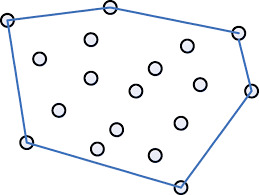
\includegraphics[scale=0.3,valign=t]{hull}
      &
  The \textit{convex hull} of a set of 2D points is a subset of the points that forms a \href{https://en.wikipedia.org/wiki/Convex_polygon}{convex polygon} which contains all the other points. It can be described informally as, the shape enclosed by a rubber band stretched around the points. 
  \end{tabularx}
  \begin{parts}
  \part[10] Design a divide and conquer algorithm to compute the convex hull of a set of 2D points and describe it using the pseudocode conventions listed in Section 2.1 of CLRS.
    \begin{solution}
\begin{codebox}
\Procname{$\proc{convex-hull}(P, n)$}
\li \If $\attrib{P}{size} \le 3$
\Then
\li \Return $P$
\End
\li $L, R \gets $ split $P$ into two halves, e.g. left and right halves
\li $\id{LH} \gets \proc{convex-hull}(L, \attrib{L}{size})$
\li $\id{RH} \gets \proc{convex-hull}(R, \attrib{R}{size})$
\li \Return \proc{merge-hulls}(\id{LH}, \id{RH})
\end{codebox}

The logic for \proc{merge-hulls} is easily available online, e.g. using tangents as described \href{https://ocw.mit.edu/courses/6-046j-design-and-analysis-of-algorithms-spring-2015/7463c413c944ed72b46a3c3d02b49448_MIT6_046JS15_lec02.pdf}{here}.
    \end{solution}
  \part[5] Visualize the running of your algorithm as an \href{https://matplotlib.org/stable/users/explain/animations/animations.html}{animation} and submit the animation as an MP4 file.
  \end{parts}
  
\end{questions}

\end{document}

%%% Local Variables:
%%% mode: latex
%%% TeX-master: t
%%% End:
